%---------------------------------------------------------------------
\begin{frame}{Recap on health insurance}
    We have covered several topics on health insurance:
    \begin{itemize}
        \item Why do people buy health insurance? {\footnotesize {\color{gray} (risk-aversion, expected utility, certainty equivalent, risk-premium, etc.)}} \pause
        \item What do health insurance plans look like and how to choose among them? {\footnotesize {\color{gray} (premiums, deductibles, copayments, coinsurance, out-of-pocket maximum, etc.)}} \pause
        \item What is moral hazard? {\footnotesize {\color{gray} (RAND experiment, Oregon Health Insurance experiment)}} \pause
        \item How to deal with moral hazard in health insurance? {\footnotesize {\color{gray} (coinsurance, deductibles, prior-authorization \& which type of care is cut)}} \pause
        \item Imperfect information and adverse selection on health insurance markets
    \end{itemize}

\end{frame}
%---------------------------------------------------------------------
\begin{frame}{Recap on health insurance}
    We have covered several topics on health insurance:
    \begin{itemize}
        \item Why do people buy health insurance?
        \item What do health insurance plans look like and how to choose among them?
        \item What is moral hazard?
        \item How to deal with moral hazard in health insurance?
        \item Imperfect information and adverse selection on health insurance markets
        \begin{itemize}
            \item Two models to think about it {\footnotesize {\color{gray} (EF (2011) and RS (1976))}}
            \item Empirical evidence {\footnotesize {\color{gray} (Huntington disease, the MA 2006 mandate, Harvard death spiral, risk-adjustment in the ACA)}} 
            \item Policies to deal with adverse selection {\footnotesize {\color{gray} (community ratings, mandate, risk-adjustment and reinsurance)}}
        \end{itemize}
        % Point out that adverse selection makes it so that even with perfect competition, the market will end on an inefficient provision because of adverse selection
        % Market failure and government intervention
    \end{itemize}
    \pause

    \vspace{3mm}

    \newbold{Today: What does health insurance do?}


\end{frame}
%---------------------------------------------------------------------
\begin{frame}{What we already know}
    
    What does health insurance do to \newbold{healthcare utilization}?
    \only<1>{
        \vspace{25mm}
    }
    \only<2>{
        \begin{itemize}
            \item RAND experiment: more coverage $\implies$ more healthcare utilization\\
            {\color{white}
            \item[] Oregon Health Insurance experiment: gaining Medicaid coverage
            \begin{itemize}
                \item[] {\color{white}$\uparrow$ healthcare utilization}
                \item[] {\color{white}$\sim$ hospitalizations through the ER}
                \item[] {\color{white}$\uparrow$ preventive care}
                \item[] {\color{white}$\uparrow$ self-reported health}
            \end{itemize}
        }
        \end{itemize}   
    }
    \only<3>{
        \begin{itemize}
            \item RAND experiment: more coverage $\implies$ more healthcare utilization\\
            \item Oregon Health Insurance experiment: gaining Medicaid coverage
            \begin{itemize}
                \item $\uparrow$ healthcare utilization
                \item $\sim$ hospitalizations through the ER
                \item $\uparrow$ preventive care
                \item $\uparrow$ self-reported health
            \end{itemize}
        \end{itemize}   
    }

\end{frame}
%---------------------------------------------------------------------
\begin{frame}{Reading 2: what did you think}
    
    Chapter 1 from Gross and Notowidigdo (2021) \textit{What does health insurance do?} in \textit{Better Health Economics}\\
    \vspace{2mm}

    \pause

    $\implies$ What did you learn from it?

\end{frame}
%---------------------------------------------------------------------
\begin{frame}{Financial health}
    
    Back to the basics: health insurance is about your \textit{finances}\\
    $\implies$ That's why you get insured\\
    \vspace{5mm}
    \pause

    Why is it hard to study?\\
    %Selection
    %Cannot compare people with and without insurance directly because of selection
    \vspace{5mm}
    \pause

    Remember the Oregon health insurance experiment?
    % Why could study the impact of health insurance?

\end{frame}
%---------------------------------------------------------------------
\begin{frame}{OHIE: the impact of public insurance on finances}
    
    \begin{center}
        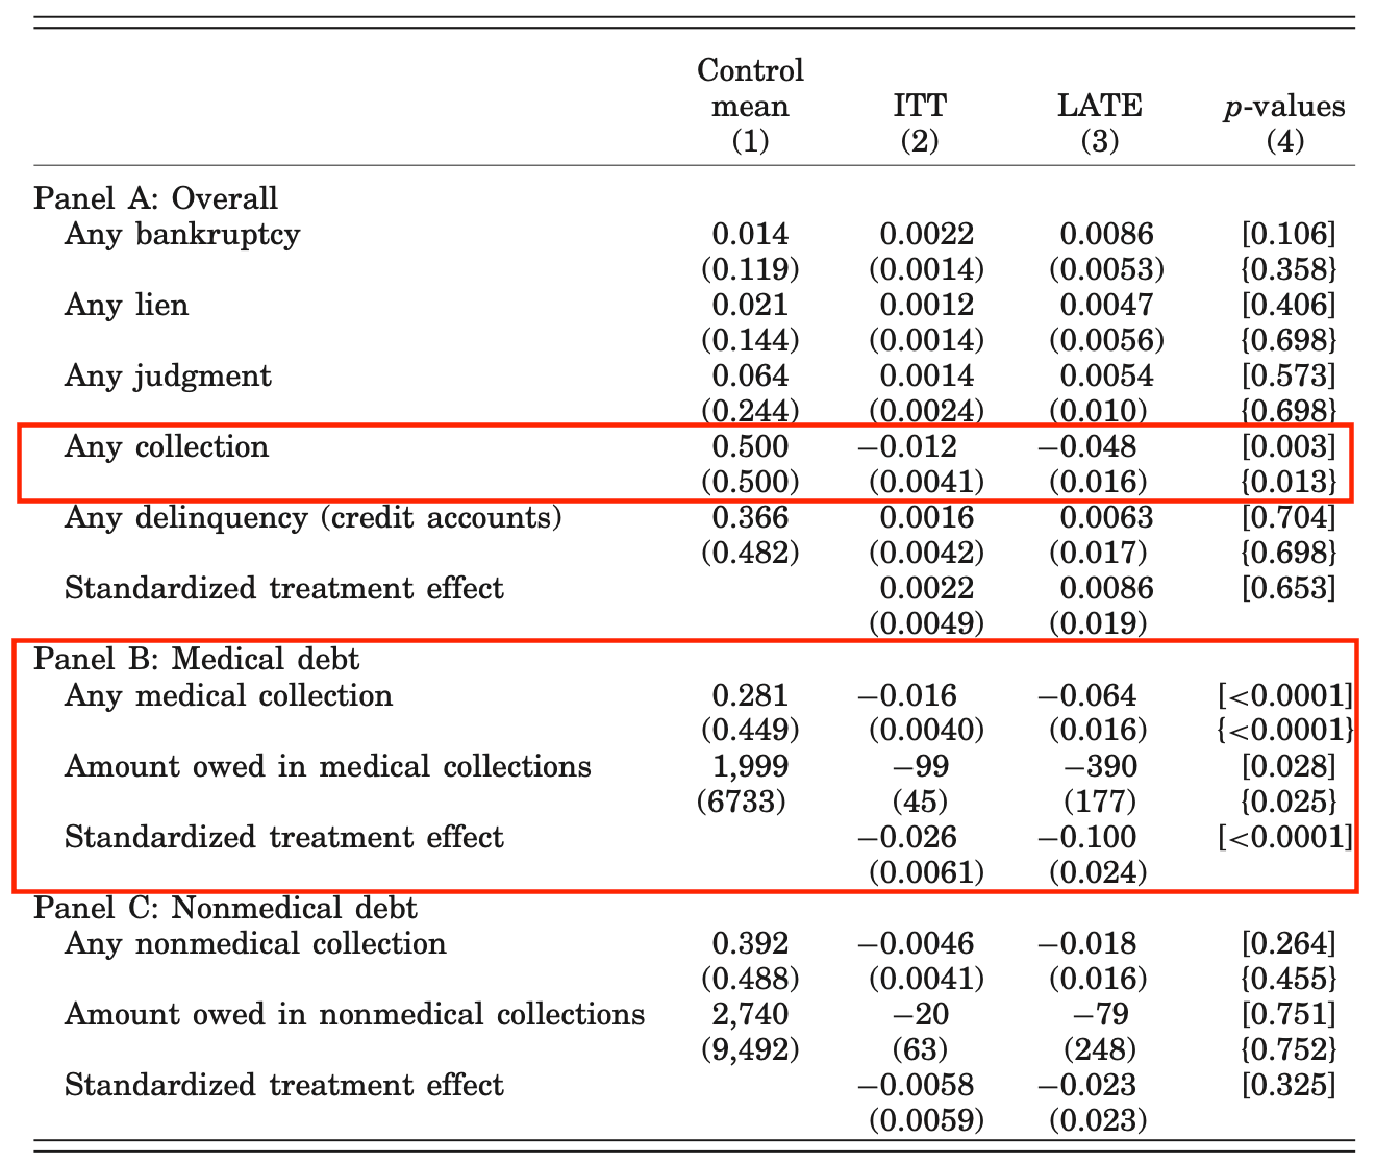
\includegraphics[height=0.9\textheight]{input/ohie_tab7.pdf}
    \end{center}    
    
\end{frame}
%---------------------------------------------------------------------
\begin{frame}{Financial health: bankruptcy rate}

    \begin{columns}
        \begin{column}{0.7\textwidth}
            \newbold{Bankruptcy}: is a legal declaration that you cannot meet your financial obligations, and a court-supervised process decides how debts are handled.
        \end{column}
        \begin{column}{0.3\textwidth}
            \begin{center}
                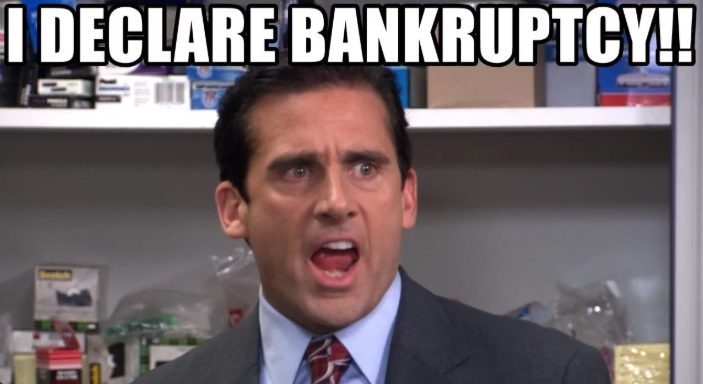
\includegraphics[width=\textwidth]{input/meme_bankruptcy.png}
            \end{center}
        \end{column}
    \end{columns}
    \vspace{2mm}
    \begin{itemize}
        \item Can't pay bills: bill collectors are calling, credit cards are maxed out
        \item Pay bankruptcy attorney who, against a fee, will file for you and represent you in court
        \item Judge decides how to divide your assets among your creditors. If no asset, debt wept away
        \item ``Fresh start''? Not fully: credit scores are low and don't recover for years
    \end{itemize}

    % Give the story about the paper: Tal and Matt as grad students at MIT in 2006
    % Hard to transition to research, lunches in Kendall square, iterating with advisors
    % Uninsured ==> Bankrupcy. Was it true?
    % How to study this?
    
    
\end{frame}
%---------------------------------------------------------------------
\begin{frame}{Financial health: bankruptcy rate}
    
    \begin{center}
        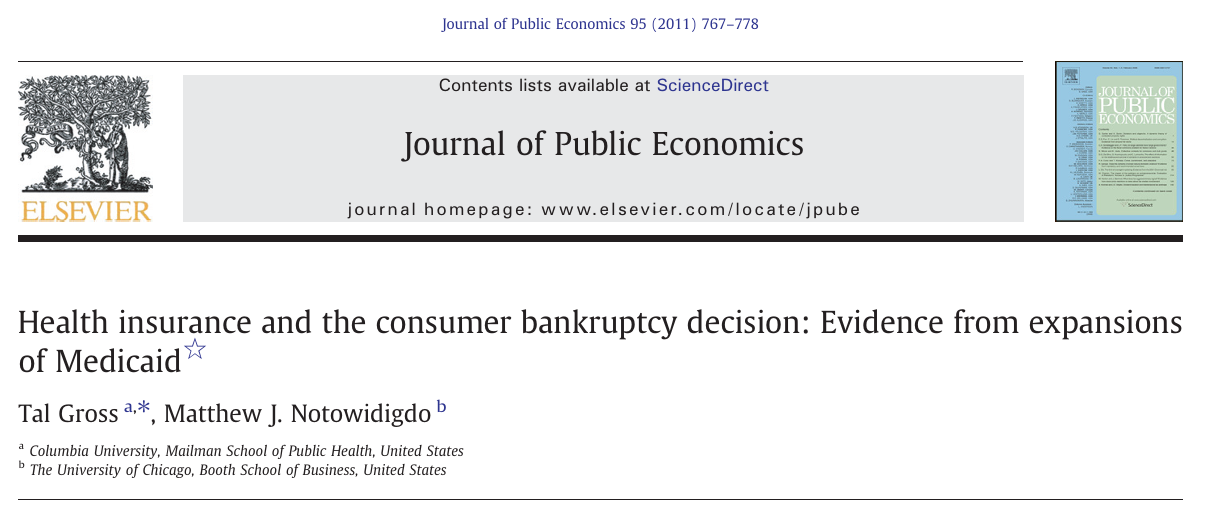
\includegraphics[height=0.75\textheight]{input/GN2011_front.png}
    \end{center}

    
\end{frame}
%---------------------------------------------------------------------
\begin{frame}{Gross and Notowidigdo (2011): financial health}
    
    How to study this?
    \begin{itemize}
        \item Medicaid expansions over time decided by states in the 90s\\
        $\implies$ \textit{Exogenously} give more public health insurance
        %When an issue? If expansions are related to economic conditions in the state.

        \vspace{2mm}

        \item Use the \textit{simulated} eligibility for Medicaid as a measure of the generosity of the program in each state and year\\
        \textit{Why not actual eligibility in a state?}\\
        \pause
        \vspace{5mm}
        Economic factors may make people more likely to become eligible for Medicaid because poorer and also more likely to be bankrupt\\
        \newbold{but} this would have nothing to do with health insurance\\
        $\implies$ Use simulated generosity instead
        % Economic crisis, more likely to be eligible for Medicaid, more likely to be bankrupt ==> correlation taht is not causal
    \end{itemize}


\end{frame}
%---------------------------------------------------------------------
\begin{frame}{Financial health: bankruptcy rate}
    
    \begin{center}
        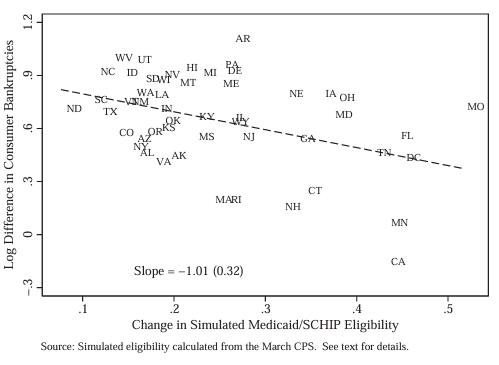
\includegraphics[height=0.85\textheight]{input/GN2011_fig3.png}
    \end{center}

    % Simulated: not actual eligibilit but simulated based on the programs rules on national sample
    % ``We also perform a similar procedure to calculate simulated eligibility. Specifically, we take a 20% national sample from the 1996 CPS and calculate the share of this fixed population that would be eligible for Medicaid in each state and year.''
    % Why? Because some economic factors may make people more likely to become eligible for Medicaid because poorer and also more likely to be bankrupt
    
\end{frame}
%---------------------------------------------------------------------
\begin{frame}{Gross and Notowidigdo (2011): findings}
    
    Does more public health insurance reduce bankruptcy?
    \begin{itemize}
        \item \newbold{Yes}: more public health insurance $\implies$ lower bankruptcy rates
        \item Magnitude: 10 percentage point increase in Medicaid eligibility reduces personal bankruptcies by 8\%
    \end{itemize}


\end{frame}
%---------------------------------------------------------------------
\begin{frame}{Dobkin, Finkelstein, Kluender, Noto (2018): people in crisis}
    
    Another way to look at it:\\
    $\implies$ What does health insurance do for your finances when you have a health crisis?\\
    \vspace{5mm}

    \begin{center}
        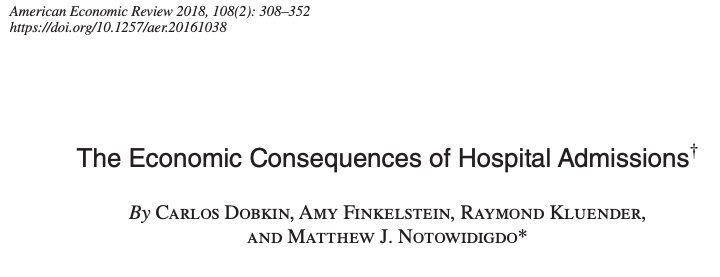
\includegraphics[height=0.55\textheight]{input/DFKN2018_front.png}
    \end{center}
\end{frame}
%---------------------------------------------------------------------
\begin{frame}{Dobkin, Finkelstein, Kluender, Noto (2018): people in crisis}
    
    What does health insurance do for your finances when you have a health crisis?\\
    \vspace{5mm}

    How?
    \begin{itemize}
        \item Large sample of hospital admissions data from California 2003-2007
        \item Link to credit report data 2002-2011
    \end{itemize}
    $\implies$ Compare the finances of people before and after a health crisis, and how it differs for people with and without insurance

\end{frame}
%---------------------------------------------------------------------
\begin{frame}{Financial health after a health crisis: insured versus uninsured}
    
    \begin{center}
        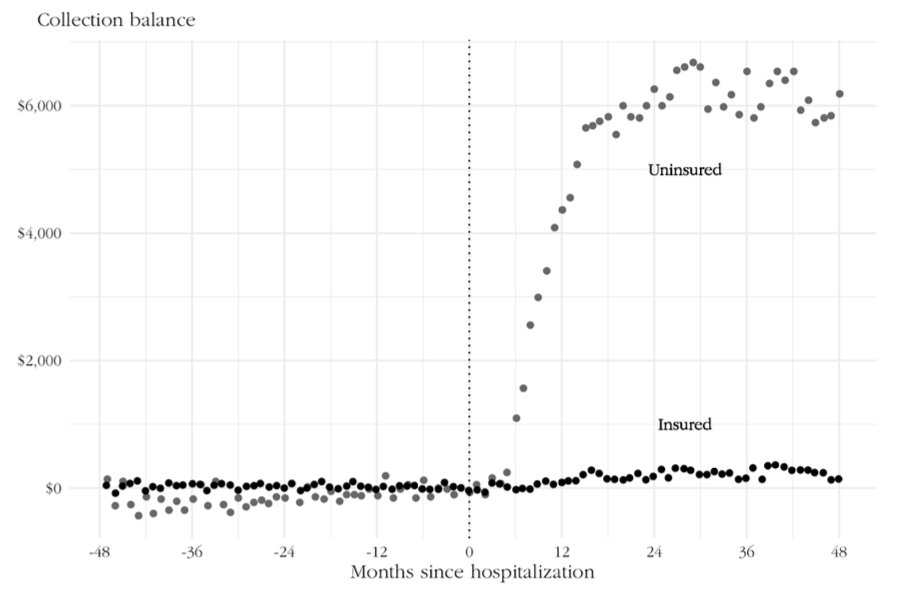
\includegraphics[height=0.85\textheight]{input/GNbook_chap1fig1.png}
    \end{center}

\end{frame}
%---------------------------------------------------------------------
% \begin{frame}{Financial health after a health crisis}
    
%     \begin{center}
%         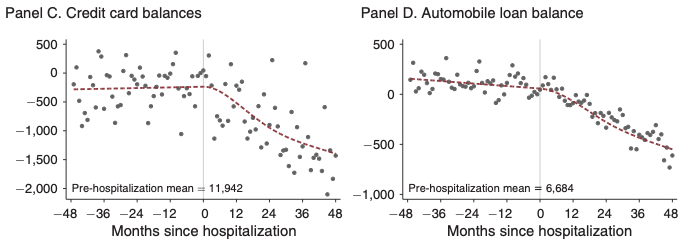
\includegraphics[height=0.6\textheight]{input/DFKN2018_fig4.png}
%     \end{center}

% \end{frame}
%---------------------------------------------------------------------
\begin{frame}{Summary: impact of health insurance on financial health}
    
    Having health insurance improves \newbold{financial health}
    \begin{itemize}
        \item Reduces personal bankruptcy rates (Gross and Notowidigdo, 2011)
        \item Reduces unpaid bills after a health crisis (Dobkin, Finkelstein, Kluender, Notowidigdo, 2018)
        \item Reduces collections (Oregon Health Insurance Experiment)
        \item[] +\textit{many other studies}
    \end{itemize}
    \vspace{3mm}

    %A WORD ON MEDICAL DEBT RELIEF?

\end{frame}
%---------------------------------------------------------------------
\begin{frame}{Impact of health insurance so far}
    
    
What does health insurance do?
\begin{itemize}
    \item More health insurance $\implies$ more healthcare utilization
    \item More health insurance $\implies$ better financial health
    \item Impact on \newbold{health}?
\end{itemize}

\end{frame}
%---------------------------------------------------------------------
\begin{frame}{The letters from the IRS}
    
    ACA mandate: you have to have health insurance or pay a tax penalty ($\sim$ \$100 in 2014, $\sim$\$300 in 2015)
    %Undone by the Trump administration
    \begin{itemize}
        \item For people who were penalized, send a letter to inform them:\\
        (1) that they paid a penalty and (2) how to avoid it next year
        \pause
        \item Limited budget to send letters: cannot send to all (but still can send to 4.5 million Americans)\\
        \pause
        $\implies$ randomized who received the letter among penalty payers (yay!)\\
        \pause
        \textit{Why is is great? Because it allows us to study the impact of health insurance on health in a randomized way!}
    \end{itemize}
    \vspace{3mm}
    \pause

    %Note: in OHIE, lottery is teh instrument for insured. Here, receiving teh letter is teh instrument for insured.

    Key: Were people who received the letter more likely to get health insurance?\\
    $\implies$ Yes, 1\% more likely
    % IS it small or large? Not bad, because its only a letter.

\end{frame}
%---------------------------------------------------------------------
\begin{frame}{Goldin, Lurie, McCubbin (2021)}

    \begin{center}
        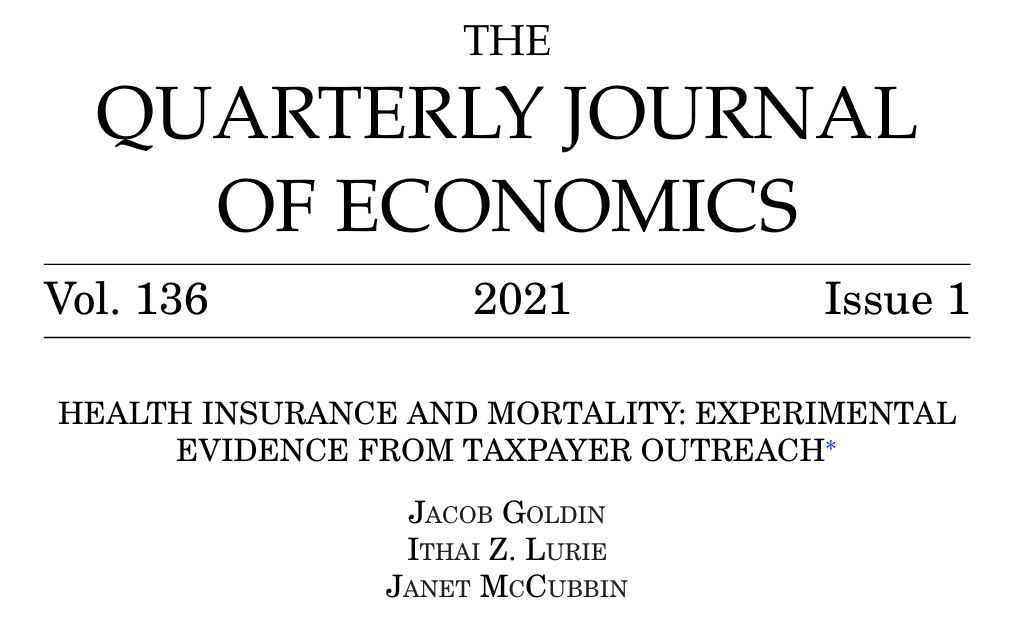
\includegraphics[height=0.85\textheight]{input/GLM2021_front.png}
    \end{center}
    
\end{frame}
%---------------------------------------------------------------------
\begin{frame}{Impact of health insurance on mortality}
    

    \begin{center}
        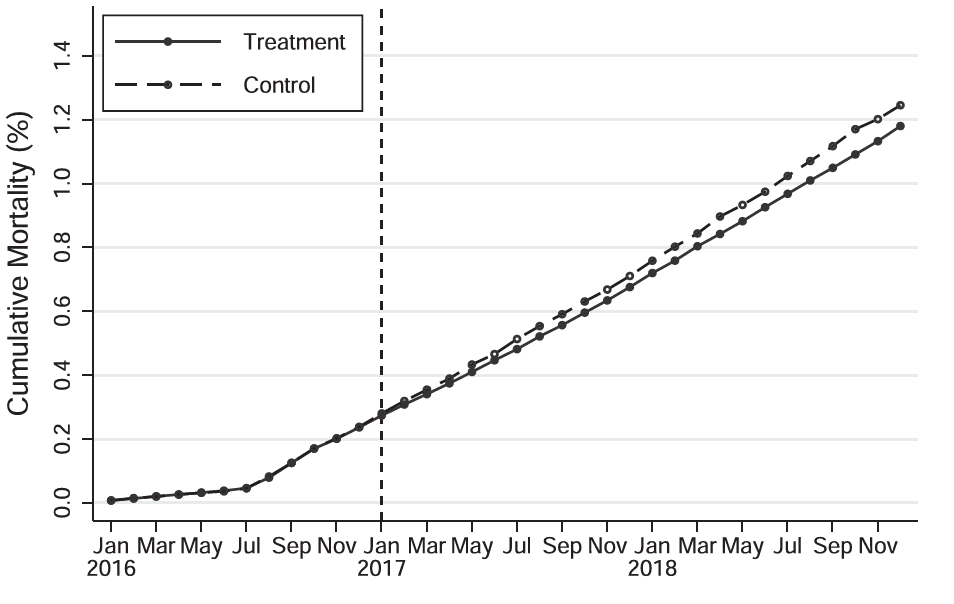
\includegraphics[height=0.85\textheight]{input/GLM2021_fig3.png}
    \end{center}
    \vspace{-4mm}
    \only<2>{Mortality rate decline of 0.5\% $\implies$ 28\% reduction in mortality}
    

\end{frame}
%---------------------------------------------------------------------
\begin{frame}{Card, Dobkin, and Maestas (2009)}
    
Does health insurance increase your chances of survival when you have a health crisis?

\begin{center}
    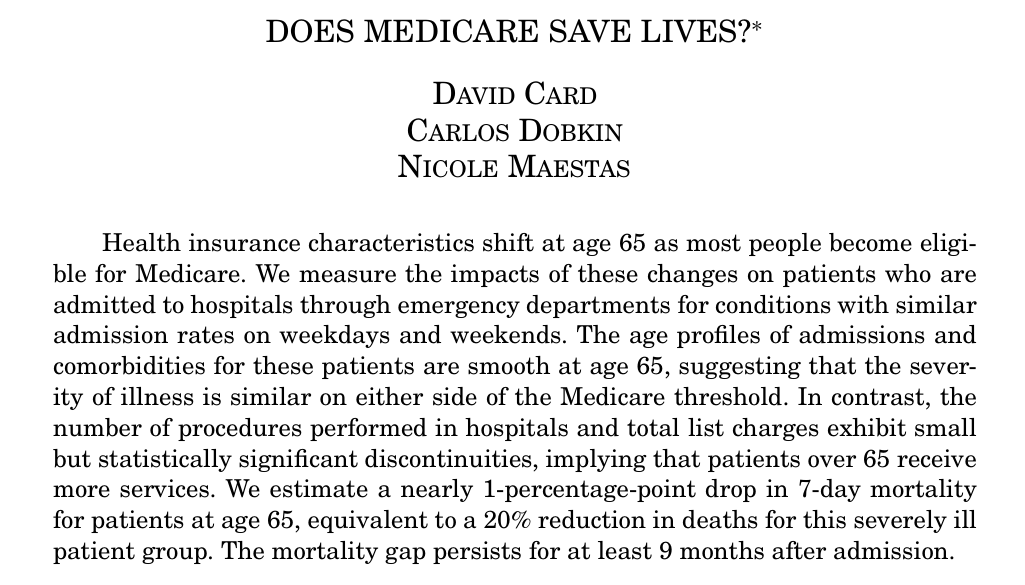
\includegraphics[height=0.75\textheight]{input/CDM2009_front.png}
\end{center}

\end{frame}
%---------------------------------------------------------------------
\begin{frame}{Card, Dobkin, and Maestas (2009)}
    
Does health insurance increase your chances of survival when you have a health crisis?\\
\vspace{3mm}

How to study this? {\footnotesize {\color{gray} (again, cannot just compare insured and uninsured because of selection)}}
\begin{itemize}
    \item Medicare: gains health insurance at age 65
    \pause
    \item What if we compared people going to the ER right before versus right after their 65th birthday?\\
    \pause
    $\implies$ Why does it help address selection?
\end{itemize}

\end{frame}
%---------------------------------------------------------------------
\begin{frame}{Card, Dobkin, and Maestas (2009)}
    
Does health insurance increase your chances of survival when you have a health crisis?\\
\vspace{3mm}

What if we compared people going to the ER right before versus right after their 65th birthday: why does it help address selection?
    \begin{itemize}
        \item People that are just before and just after their 65th birthday are likely to be very similar in terms of health, income, etc.
        \pause
        \item The key difference: more likely to be insured after their 65th birthday
        \pause
    \end{itemize}
    $\implies$ We can attribute any difference in mortality to the impact of health insurance (Medicare in particular here)\\
    \pause
    This empirical strategy is called a \newbold{regression discontinuity design}

% \vspace{3mm}
%  Data: 1992 to 2002 in California

\end{frame}
%---------------------------------------------------------------------
\begin{frame}{Card, Dobkin, and Maestas (2009): why such an impact?}
    
Does health insurance increase your chances of survival when you have a health crisis?\\
$\implies$ \newbold{Yes.} $\sim$ 1-percentage-point drop in 7-day mortality for patients at age 65\\
\vspace{3mm}
\pause

\newbold{But why??} The truth is that it is not clear
\begin{itemize}
    \item Patients after 65 receive more procedures
    \begin{itemize}
        \item Maybe patients are more likely to seek care when insured
        \item Maybe doctors are more likely to provide care when patients are insured
        %Maybe Medicare has beter coverage?
    \end{itemize}
\end{itemize}

\end{frame}
%---------------------------------------------------------------------
\begin{frame}{Card, Dobkin, and Maestas (2009): why such an impact?}
    
\begin{center}
    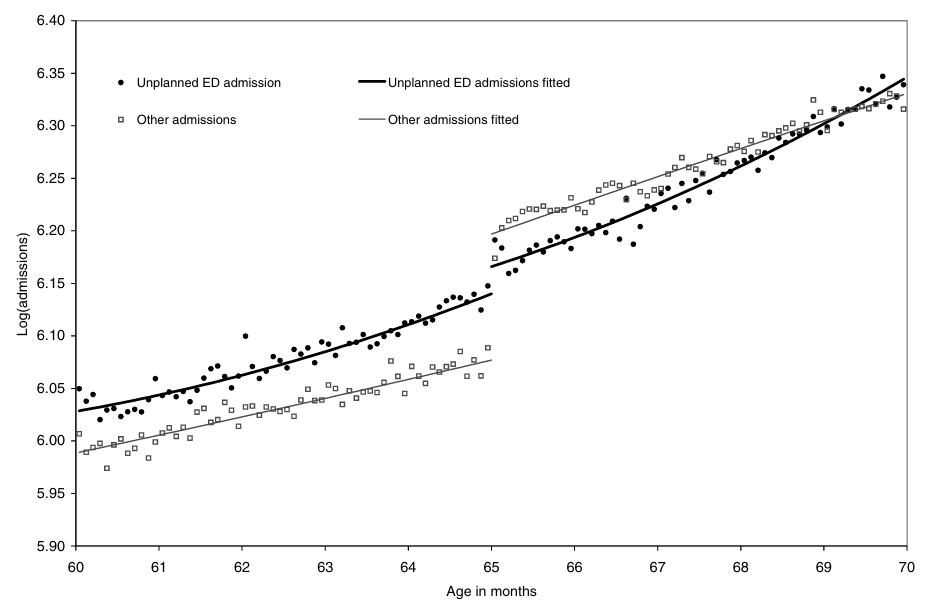
\includegraphics[height=0.85\textheight]{input/CDM2009_fig2.png}
\end{center}

%Unplanned and non-deferrable (same rate weekends and weekdays)
% What is a planned ER? after-hours, missing beds

\end{frame}
%---------------------------------------------------------------------
\begin{frame}{Conclusion: what does health insurance do?}
    
Why is it hard to study?\\
$\implies$ Who has health insurance is not random (selection)\\
\vspace{5mm}

What do we know?
\begin{enumerate}
    \item More health insurance $\implies$ more healthcare utilization
    \item More health insurance $\implies$ better financial health
    \item More health insurance $\implies$ better health (lower mortality)\\
    \textit{+ evidence on preventive care, self-reported health, etc.}
\end{enumerate}

\end{frame}
%---------------------------------------------------------------------
\begin{frame}{Conclusion: what does health insurance do?}
    
Because health insurance has many advantages $\implies$ we really care about making sure everyone has access to it\\
\vspace{7mm}


Why would the government get involved though?\\
\textit{i.e., why is it different from broccoli (cf Gross and Noto's book) ?}\\
%Brocolli is also good for you but the government doesn't force oyu to eat it. What's different?
\only<1>{
    \vspace{5mm}
}
\only<2>{
    $\implies$ Adverse selection + asymmetry of information: market failure \\
}

% Market failure is even more important based on the high value of health insurance

\end{frame}
%---------------------------------------------------------------------
\begin{frame}{}
    \begin{center}
    \Large \textcolor{maroon}{Wrapping up}
    \end{center}
\end{frame}
%---------------------------------------------------------------------
\begin{frame}{To next class}
\begin{itemize}
    \item \newbold{TO DO}
    \begin{enumerate}
        \item \newbold{Problem set 4} posted: due \newbold{Thursday March 26th by 9:30am}
        \item Review this class and past material $\implies$ \textit{questions on it?}
    \end{enumerate}
    \vspace{5mm}

    \item Program for next class
    \begin{itemize}
        \item The Affordable Care Act
    \end{itemize}
\end{itemize}
\end{frame}
%---------------------------------------------------------------------